99. \begin{figure}[ht!]
\center{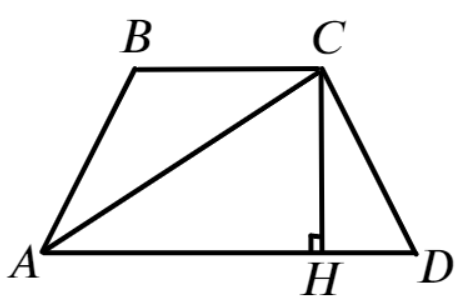
\includegraphics[scale=0.35]{g9-99.png}}
\end{figure}\\
Так как трапеция описанная, суммы её противоположных сторон равны, значит $AB=CD=\cfrac{a+b}{2}.$ Пусть $b>a.$ Опустим высоту $CH,$ тогда $HD=\cfrac{b-a}{2}$ и $CH^2=\cfrac{a^2+2ab+b^2}{4}-\cfrac{a^2-2ab+b^2}{4}=ab,\ AH=b-\cfrac{b-a}{2}=\cfrac{a+b}{2},\ AC=\sqrt{\cfrac{a^2+2ab+b^2}{4}+ab}=\cfrac{1}{2}\sqrt{a^2+6ab+b^2}.$
ewpage
oindent
